 \documentclass[a4paper]{tufte-book}
\usepackage{booktabs}
\usepackage{tabularx}
\usepackage{longtable} 
\usepackage{lscape}
\usepackage{colortbl}
\usepackage{graphicx}
\graphicspath{ {../images/} }

%\geometry{
%  left=.5in,
%  right=.5in,
%  top=.5in,
%  bottom=.5in
%}

\title{Toolkit: Hierarchical Control Model Picture}

\begin{document}

\setlength{\parindent}{0em}
\setlength{\parskip}{.75em}


\section{Hierarchical Control Model Starting Point}

\begin{fullwidth}
\newthought{Starting Questions}

\begin{itemize}
\setlength{\itemsep}{0pt}
\setlength{\parskip}{.25em}
\item What are some of the participants? (names of groups, components, etc.)
\item What responsibilities are present here? Whose are they?
\item What actions are available? Whose are they?
\item What decisions are being made and who or what is responsible for making them?
\item What information do components use to make those decisions, and how do they get it?
\end{itemize}

\newthought{Visual Conventions}

\begin{itemize}
\setlength{\itemsep}{0pt}
\setlength{\parskip}{.25em}
\item Items higher on the page exercise authority over the things lower on the page.
\item Arrows pointing down represent \emph{control actions} or exerting \emph{authority}.
\item Arrows pointing up represent \emph{feedback} via sensors, also describable as \emph{accountability}.
\item Horizontal lines represent coordination and handoffs.
\item Boxes may be nested, representing sub-processes.
\end{itemize}

\begin{center}
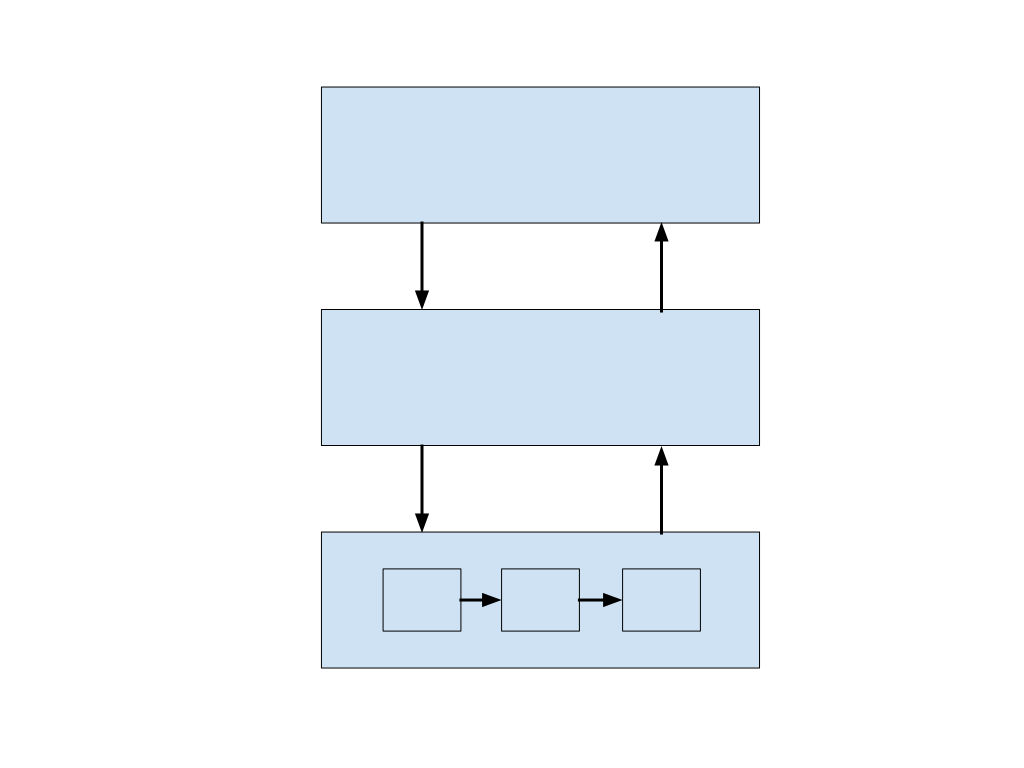
\includegraphics[width=10cm]{generic_model.png}
\end{center}

\end{fullwidth}
\end{document}